\documentclass[tikz,border=10pt]{standalone}
\usetikzlibrary{positioning, arrows.meta}

\colorlet{green_set}{green!70!black}
\colorlet{purple_set}{blue!80!cyan!60!red!95!black!90}
\colorlet{red_set}{red!80!black}

\begin{document}
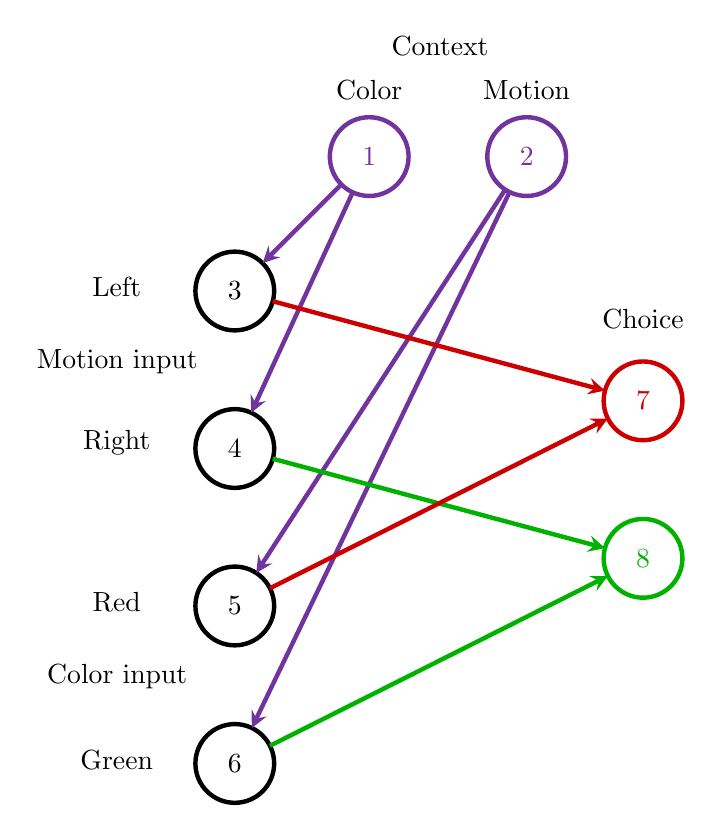
\begin{tikzpicture}[neuron/.style={circle, draw, minimum size=1cm, inner sep=0pt, outer sep=0pt, ultra thick},
                    connection/.style={->, >=stealth, ultra thick},
                    label distance=3mm] 

  % Define neurons
  \node[purple_set, neuron, label={[xshift=0.0cm, yshift=-0.2cm]Color}] (n1) {1};
  \node[purple_set, neuron, label={[xshift=0.0cm, yshift=-0.2cm]Motion}] (n2) [right=of n1] {2};
  \node[neuron, label={[xshift=-1.5cm, yshift=-1.0cm]Left}] (n3) [below left=of n1] {3};
  \node[neuron, label={[xshift=-1.5cm, yshift=-1.0cm]Right}] (n4) [below=of n3] {4};
  \node[neuron, label={[xshift=-1.5cm, yshift=-1.0cm]Red}] (n5) [below=of n4] {5};
  \node[neuron, label={[xshift=-1.5cm, yshift=-1.0cm]Green}] (n6) [below=of n5] {6};
  \node (n_ghost) [below right=of n2] {}; % Invisible node for spacing
  \node[red_set, neuron, label=above:Choice] (n7) [below=of n_ghost] {7};
  \node[green_set, neuron] (n8) [below=of n7] {8};

  % Connections
  \draw[purple_set, connection] (n1) -- (n3);
  \draw[purple_set, connection] (n1) -- (n4);
  \draw[purple_set, connection] (n2) -- (n5);
  \draw[purple_set, connection] (n2) -- (n6);
  \draw[red_set, connection] (n3) -- (n7);
  \draw[green_set, connection] (n4) -- (n8);
  \draw[red_set, connection] (n5) -- (n7);
  \draw[green_set, connection] (n6) -- (n8);

  \node[] at (-3.2,-2.6) {Motion input};
  \node[] at (-3.2,-6.6) {Color input};
  \node[] at (0.9,1.4) {Context};

\end{tikzpicture}
\end{document}